\section{Results}
\label{sect:results}
{\color{red}[TODO: perhaps heading should be ``Data Analysis'' -- or perhaps two sections?]}

{\color{red}
Presentation of analysis methods in an incremental/progressive manner:
\begin{enumerate}
\item Timeseries plots of traffic volume reveals that \emph{some} event occurred, but does not allow for differentiation between specific events. In addition, this approach does not work for all devices.
\item Observing for phone to cloud, cloud to plug traffic allows us to determine if plug is toggled from home or afar (assuming phone has wifi enabled) for some plugs (those which are exclusively controlled by the cloud server).
\item Observing lengths of packets exchanged between phone, cloud, and plug (coupled with DNS request+response+subsequent connection to IP) reveals the occurrence of specific events for some devices.
\end{enumerate}
}

\begin{figure}
  \caption{SmartThings Plug toggled ON using a phone connected to the local network.}
  \label{fig:st-plug-on-local-phone}
  \centering
    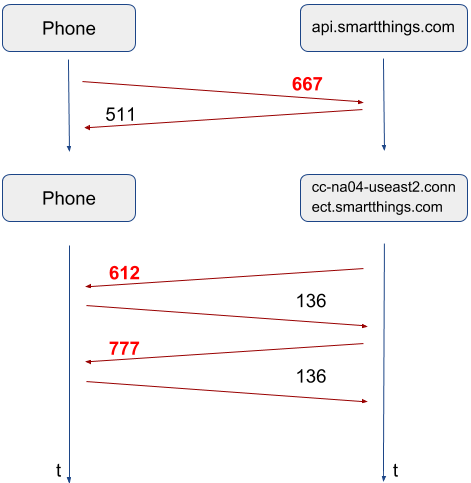
\includegraphics[width=0.5\linewidth]{figures/ST-plug-ON-local-phone.png}
\end{figure}

\begin{figure}
  \caption{SmartThings Plug toggled OFF using a phone connected to the local network.}
  \label{fig:st-plug-off-local-phone}
  \centering
    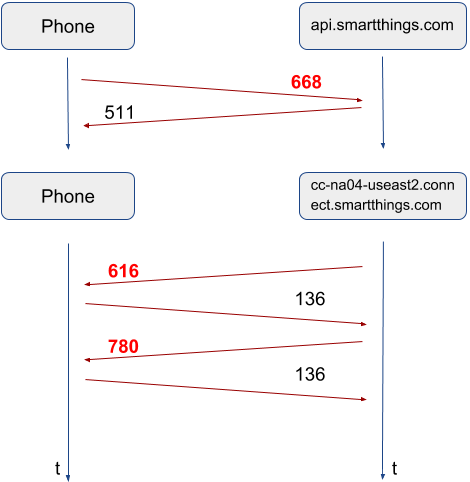
\includegraphics[width=0.5\linewidth]{figures/ST-plug-OFF-local-phone.png}
\end{figure}


% below subfigure style should be possible once we figure out how to include subcaption package.
%\begin{figure}
%\begin{minipage}[b]{0.5\textwidth}
%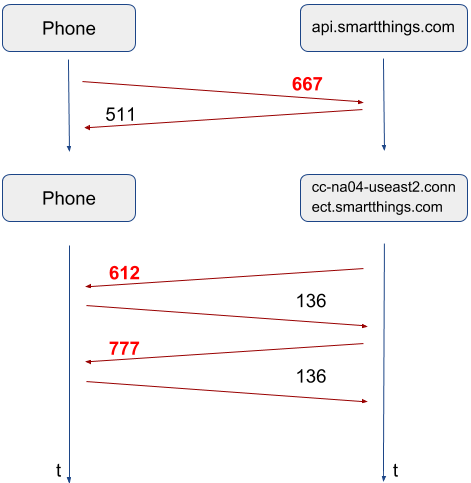
\includegraphics{figures/ST-plug-ON-local-phone.png}\\
%\subcaption{A subfigure}
%\end{minipage}%
%\begin{minipage}[b]{0.5\textwidth}
%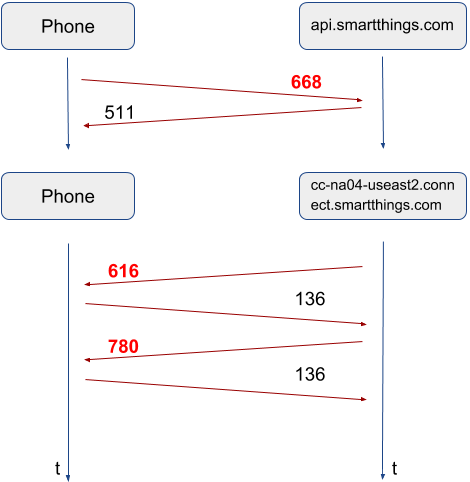
\includegraphics{figures/ST-plug-OFF-local-phone.png}\\
%\subcaption{Another subfigure}
%\end{minipage}%
%\caption{Several figures}
%\end{figure}